\begin{figure*}
  \centering
  %\begin{subfigure}{0.32\textwidth}
  %  \includegraphics[width=\textwidth]{figures/pdfs/PersistLatencyThroughput/TATP.pdf}
  %  \caption{TATP}
  %  \label{fig::PersistLatencyThroughput::TATP}
  %\end{subfigure}
  %\begin{subfigure}{0.32\textwidth}
  %  \includegraphics[width=\textwidth]{figures/pdfs/PersistLatencyThroughput/TPCB.pdf}
  %  \caption{TPCB}
  %  \label{fig::PersistLatencyThroughput::TPCB}
  %\end{subfigure}
  %\begin{subfigure}{0.32\textwidth}
  %  \includegraphics[width=\textwidth]{figures/pdfs/PersistLatencyThroughput/TPCC.pdf}
  %  \caption{TPCC}
  %  \label{fig::PersistLatencyThroughput::TPCC}
  %\end{subfigure}
  \subfigure[TATP -- Update Location]{\label{fig::PersistLatencyThroughput::TATP} 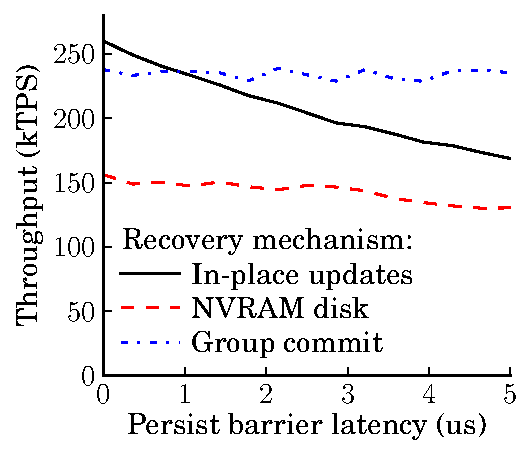
\includegraphics[width=.49\textwidth]{OLTP_eval/PersistLatencyThroughput_TATP.pdf}}
  \subfigure[TPCB]{\label{fig::PersistLatencyThroughput::TPCB}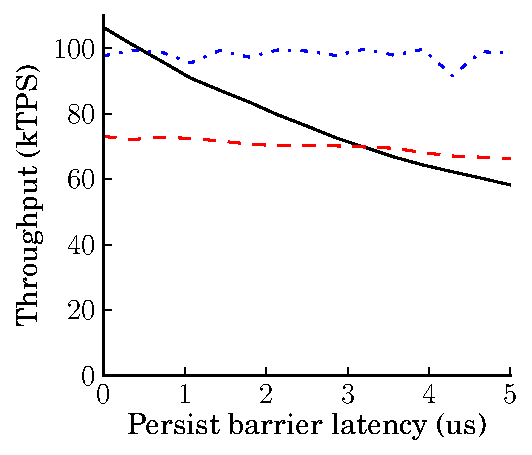
\includegraphics[width=.49\textwidth]{OLTP_eval/PersistLatencyThroughput_TPCB.pdf}}
  \subfigure[TPCC -- New Order]{\label{fig::PersistLatencyThroughput::TPCC}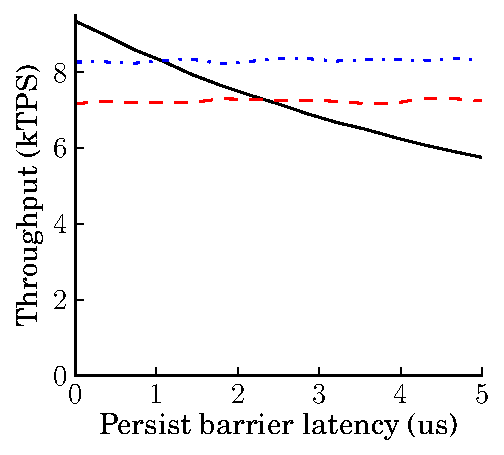
\includegraphics[width=.49\textwidth]{OLTP_eval/PersistLatencyThroughput_TPCC.pdf}}
  \caption{\textbf{Throughput vs persist barrier latency.} \InPlace performs best for zero-cost persist barriers, but throughput suffers as persist barrier latency increases.  \NVDisk and \GroupCommit are both insensitive to increasing persist barrier latency, with \GroupCommit offering higher throughput.}
  \label{fig::PersistLatencyThroughput}
\end{figure*}
